\section{Use Case Demonstration}

An example experiment was generated as a proof of concept to demonstrate a potential workflow for testing the effect of various independent variables on SfM accuracy.  This experiment specifically is generated to observe how the dense reconstruction quality setting in Agisoft Photoscan effects the resultant pointcloud accuracy.  The results suggest that a higher quality dense reconstruction setting will generate more accurate results.

\subsection{Experiment Design}
A 200 m x 200m square surface was manually generated to simulate a topography with rolling hills using a 1 meter grid.  A large 27m$^3$ meter cube was placed in the center of the scene to test surface reconstruction accuracy on regions with sharp corners and edges.  Ten 1m x 1m x 0.05m square Ground Control Points (GCPs) are distributed evenly throughout the scene 0.25 meters above the ground surface.  The material of all the objects in the scene are modeled as perfect lambertian surfaces.  The topographic surface was textured using a combination of two textures.  The first texture is a 7200x7200 pixel aerial image \todo{cite NZ} for an effective texel footprint of 2.78cm square.  The second texture is a 3456x3456 pixel image of grass was tiled ten times in both the x and the y dimension for an effective texel footprint of 0.58cm square.  The image of grass was taken with a DSLR and manually edited to create a seamless texture for tiling.  The aerial image and grass texture were merged together by setting the grass texture with an alpha of 0.15 and the aerial image layered beneath it with an alpha value of 1.  The cube was textured using a 3456x3456 pixel seamless image of rocks that was derived from a DSLR image taken by the authors.  This resulted in an effective texel footprint of 0.35cm.  Each of the textures is set so that the coloring on the scene is interpolated between texels so that there are no abnormal effects on the edge of pixels.  An aerial image and oblique image of the scene are shown in \figref{fig:scene}. \todo{make this figure better. break into 2 figures. one shows layout of cameras and GCPs, one shows close up of gcp and box}

The scene was illuminated using a "Sun" lamp where all of the light rays are parallel to each other.  The light is initially directed at nadir and is linearly interpolated to a 30 degree rotation about the x axis for the final image. The sun has a constant intensity of 1, and emits white light with values of 1 for the R,G, and B.  To improve lighting in shadowed regions, an ambient light source was added with an intensity value of 0.25 and values of 1 for R,G, and B.  

\begin{figure}[H]
	\centering
	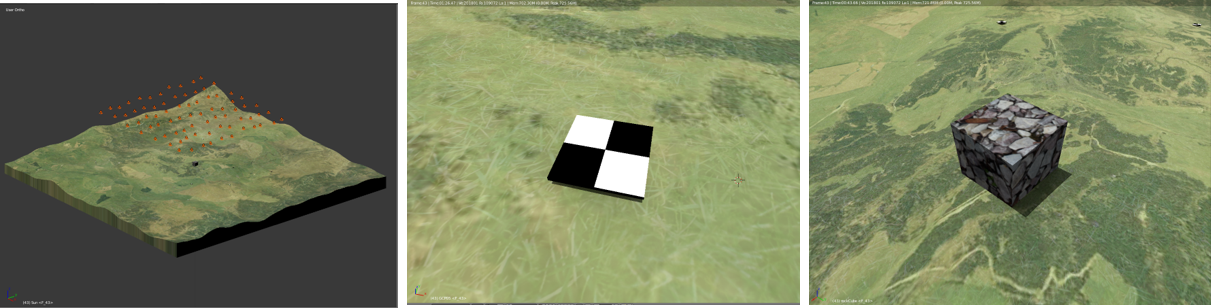
\includegraphics[height = 1.5in]{../fig/scenesummary}

	\caption{The scene was generated in Blender to represent a hilly topography with 10 Ground Control Points distributed throughout the scene and a 3m cube placed in the center.}
	\label{fig:scene}
\end{figure}

A camera is created in Blender with parameters meant to emulate a Sony A5000 with a 16mm lens and 5456x3632 pixel sensor.  A flight path is generated to create a Ground Sampling Distance (GSD) of 1.00cm and an overlap and sidelap of 75\% each.  In order to reduce imaging the edge of the simulated topographic surface, the inner 100m x 100m of the topography are selected as the Area of Interest.  Using these constraints, a trajectory consisting of 77 images distributed across 7 flight lines is generated with nadir looking imagery, as shown in \figref{fig:experimentDesign}.  In order to generate imagery that is more representative of a real world scenario with a UAS, 1 sigma gaussian noise in meters is added to the camera translation in each of the three dimensions and 2 sigma gaussian noise in degrees is added to the camera rotation about each of the three axes.  Imagery is then rendered using Blender Internal Render Engine with the default 8-sample antialiasing enabled.  \todo{how long did this take?}

\begin{figure}[H]
	\centering
	\includegraphics[height = 4in]{../fig/experimentDesign}
	\caption{}
	\label{fig:experimentDesign}
\end{figure}

The imagery that is output from Blender is postprocessed in Matlab to simulate nonlinear brown distortion \todo{cite brown distortion}, vignetting, salt/pepper noise, gaussian noise, and gaussian blur.  In order to adequately apply fisheye distortion and gaussian blur, the imagery was rendered at a larger resolution than the sensor and then cropped after the filtering was applied.  The constants used in this postprocessing are shown in \tabref{tab:postproc}  
\todo{need to add equations for brown distortion, vignetting, add distortion eqn units, etc... this could get cumbersome...}

% Table generated by Excel2LaTeX from sheet 'Parameter Distributions'
\begin{table}[htbp]
  \centering
  \caption{.}
    \begin{tabular}{lrr}
    	\toprule
    Parameter & Value & units \\
    \midrule
    Distortion $k_1$ & -4    & f \\
    Distortion $k_2$ & -4    & f \\
    Distortion $k_3$ & -4    & f \\
    Distortion $k_4$ & -4    & f \\
    Distortion $p_1$ & -4    & f \\
    Distortion $p_2$ & -4    & f \\
	Vignetting $v_1$ & 10    & DN \\	
    Vignetting $v_2$ & 0.2   & DN \\
    Vignetting $v_3$ & 0     & DN \\
    Salt Noise Probability & 0.01 & \% \\
    Pepper Noise Probability & 0.01 & \% \\
    Gaussian Noise Mean & 0 & DN \\
    Gaussian Noise Variance & 0.02 & DN \\
    Gaussian Blur Sigma & 1 & \\
    \bottomrule
    \end{tabular}%
  \label{tab:postproc}%
\end{table}%

\subsection{Processing Methodology}
The resultant imagery was processed using the commercial software Agisoft Photoscan Pro using the settings shown in \todo{cite table}.  The dataset was processed by inputting the position of the cameras, the position of the GCPs, and the camera calibration file with no uncertainty or error added.  Additionally, the pixel coordinates of the GCPs, which are traditionally clicked by the user by varying degrees of accuracy are calculated using photogrammetric equations and input into the program.  A nonlinear adjustment is performed using the "optimize" button, and the reported total RMSE for the GCPs is 0.38mm.  This represents an idealized scenario which is currently unrealistic for a real world scenario as traditionally there will be error in the GCP surveyed markers, the UAS position, the user clicking of pixel coordinates for GCPs, and in the calculation of the camera calibration.  

A dense reconstruction is performed using the "aggressive" filtering and each of the quality settings available in Photoscan.  The quality settings downsample the imagery for faster processing, and ultrahigh becomes quickly unattainable to users without purpose built CPUs with a large amount of RAM. \todo{better describe quality and cite photoscan manual}. The processing time and number of points for each pointcloud is shown in \tabref{tab:pctime}.  The computer used for this experiment is a Windows 7 Desktop PC with a Intel Xeon CPU E5-1603 @ 2.80GHz, GeForce GTX 980 Graphics card (4Gb), and 32Gb of RAM.

% Table generated by Excel2LaTeX from sheet 'Sheet7'
\begin{table}[htbp]
  \centering
  \caption{Add caption}
    \begin{tabular}{lcrrr}
   	\toprule
    Pointcloud Name & Time (Hours:Minutes) & Number of Points & RMSE Mean (m) & RMSE std (m)\\
    \midrule
    sparse          & 00:36 & 22,214       & -0.0001  & 0.0028 \\
    dense lowest    & 00:03 & 716,331      & -0.0066  & 0.0323 \\
    dense low       & 00:09 & 2,886,971    & -0.0020  & 0.0154 \\
    dense medium    & 00:30 & 11,587,504   & -0.0005  & 0.0077 \\
    dense high      & 02:19 & 46,465,218   & -0.0002  & 0.0044 \\
    dense ultrahigh & 11:54 & 186,313,448 & -0.0002  & 0.0026 \\
    \bottomrule
    \end{tabular}%
  \label{tab:pctime}%
\end{table}%


Each of the dense pointclouds is processed using CloudCompare \todo{cite} and compared to the groundtruth blender mesh using the "point to plane" tool\todo{cite}.  This tool calculates the signed distance of every point in the pointcloud to the nearest surface on the mesh, using the surface normal to determine the sign of the error. Each pointcloud was then exported and analyzed in Matlab to determine how the dense reconstruction quality setting effects the pointcloud error.

\subsection{Results}

The error was first visualized spatially for each reconstruction by gridding the pointcloud elevation and error using a nearest neighbor gridding technique.  The number of points and standard deviation of points in each grid cell are also visualized.  The results for the medium quality dense reconstruction are shown in \figref{fig:spatial}.  These plots are useful to begin to explore the spatial variability in both the density and the errors in the data.  One initial observation for this dataset is that there is a larger standard deviation of error at the edges of the pointcloud outside the extents of the AOI.  This is due to the poor viewing geometry at the edges of the scene, and suggests that in practice these data points outside of the AOI should be either discarded or used cautiously.

\begin{figure}[H]
	\centering
	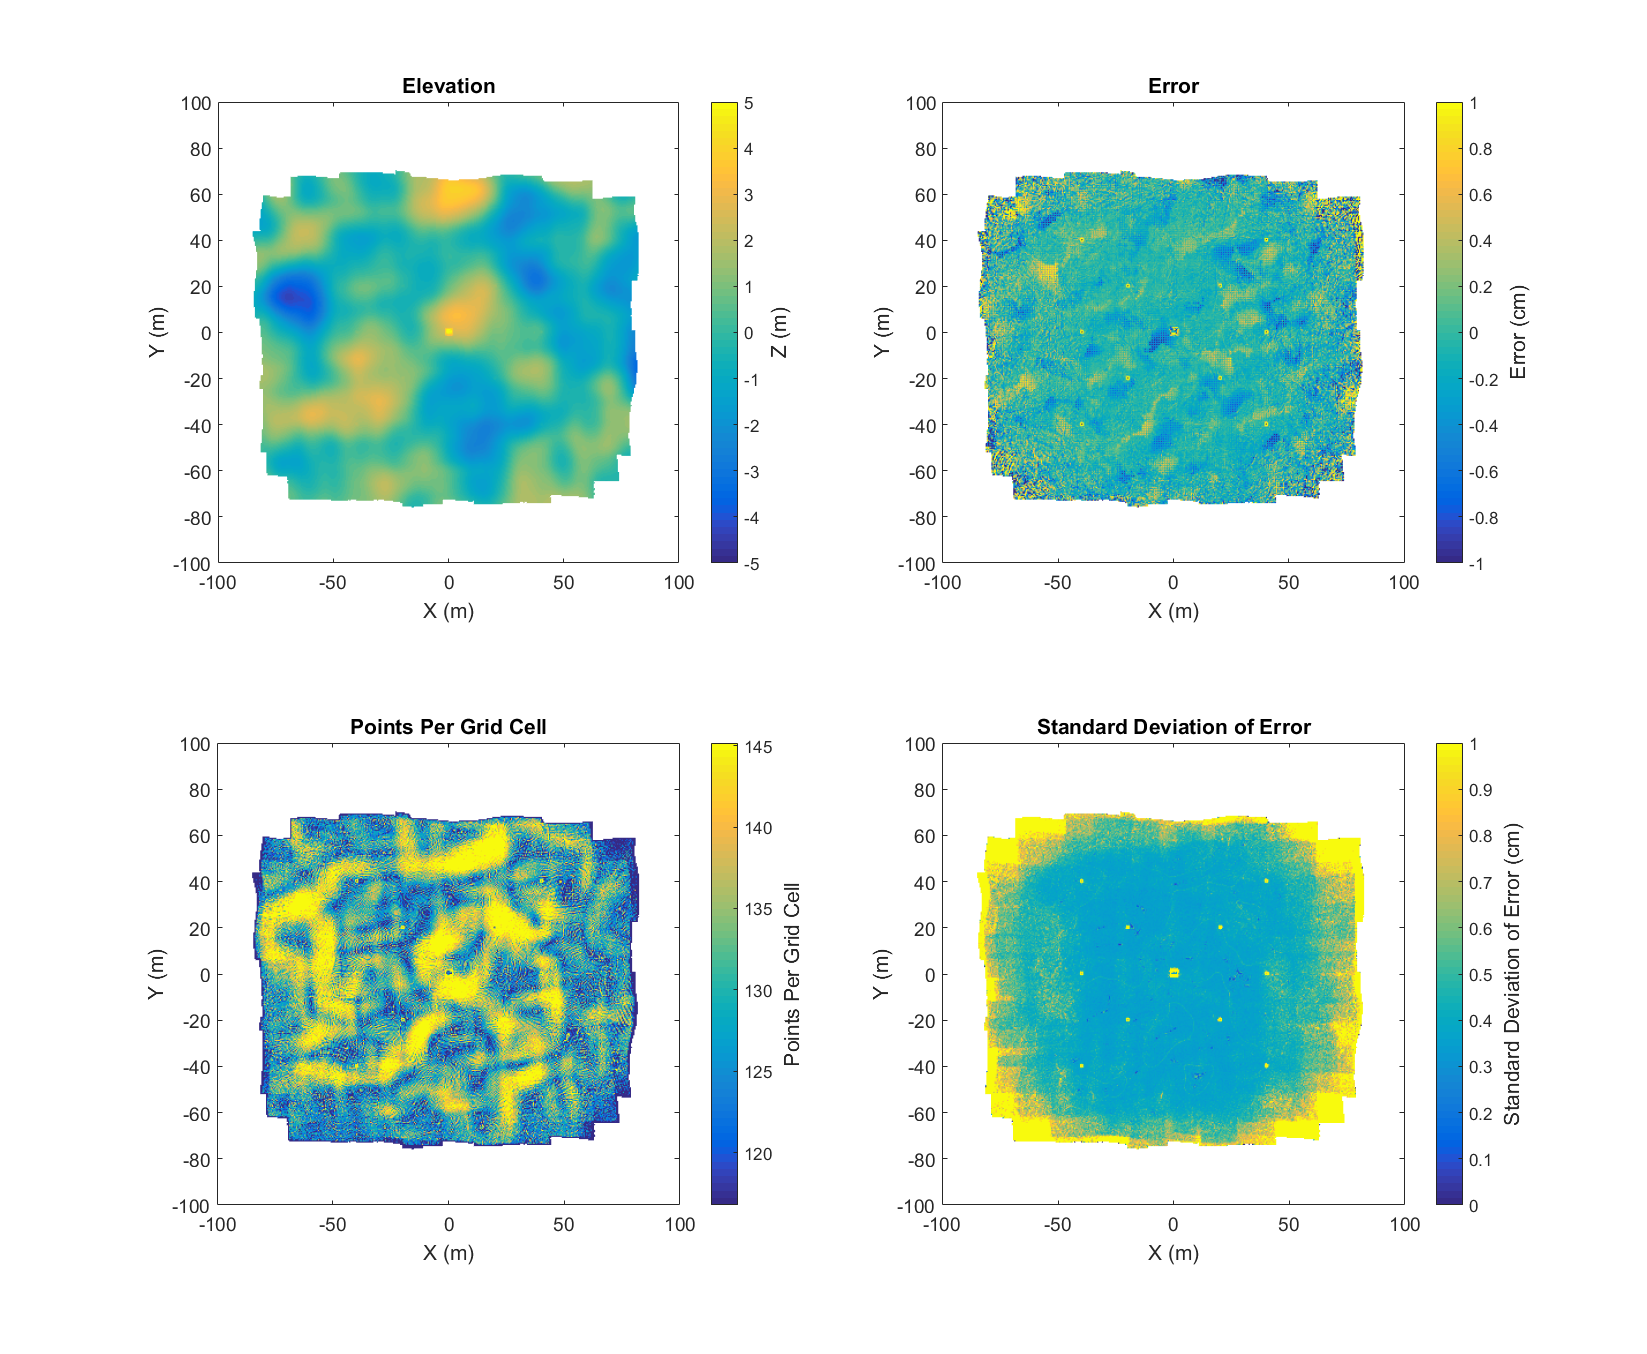
\includegraphics[height = 5in]{../fig/spatialmedium}

	\caption{The elevation, error, number of points, and standard deviation of error are gridded to 0.5 meter grid cells using a nearest neighbor gridding algorithm and visualized.}
	\label{fig:spatial}
\end{figure}

To qualitatively observe the effect of different quality dense reconstructions, a plot showing the true surface and the points from each construction in a 0.5 meter wide section of the 27m$^3$ box is shown in \figref{fig:boxplot}.  Notice that the accuracy of each pointcloud at the sharp corners of the box improves as the quality of the reconstruction increases.  This observation suggests that higher quality dense reconstruction settings will increase accuracy in regions with sharp corners.

\begin{figure}[H]
	\centering
	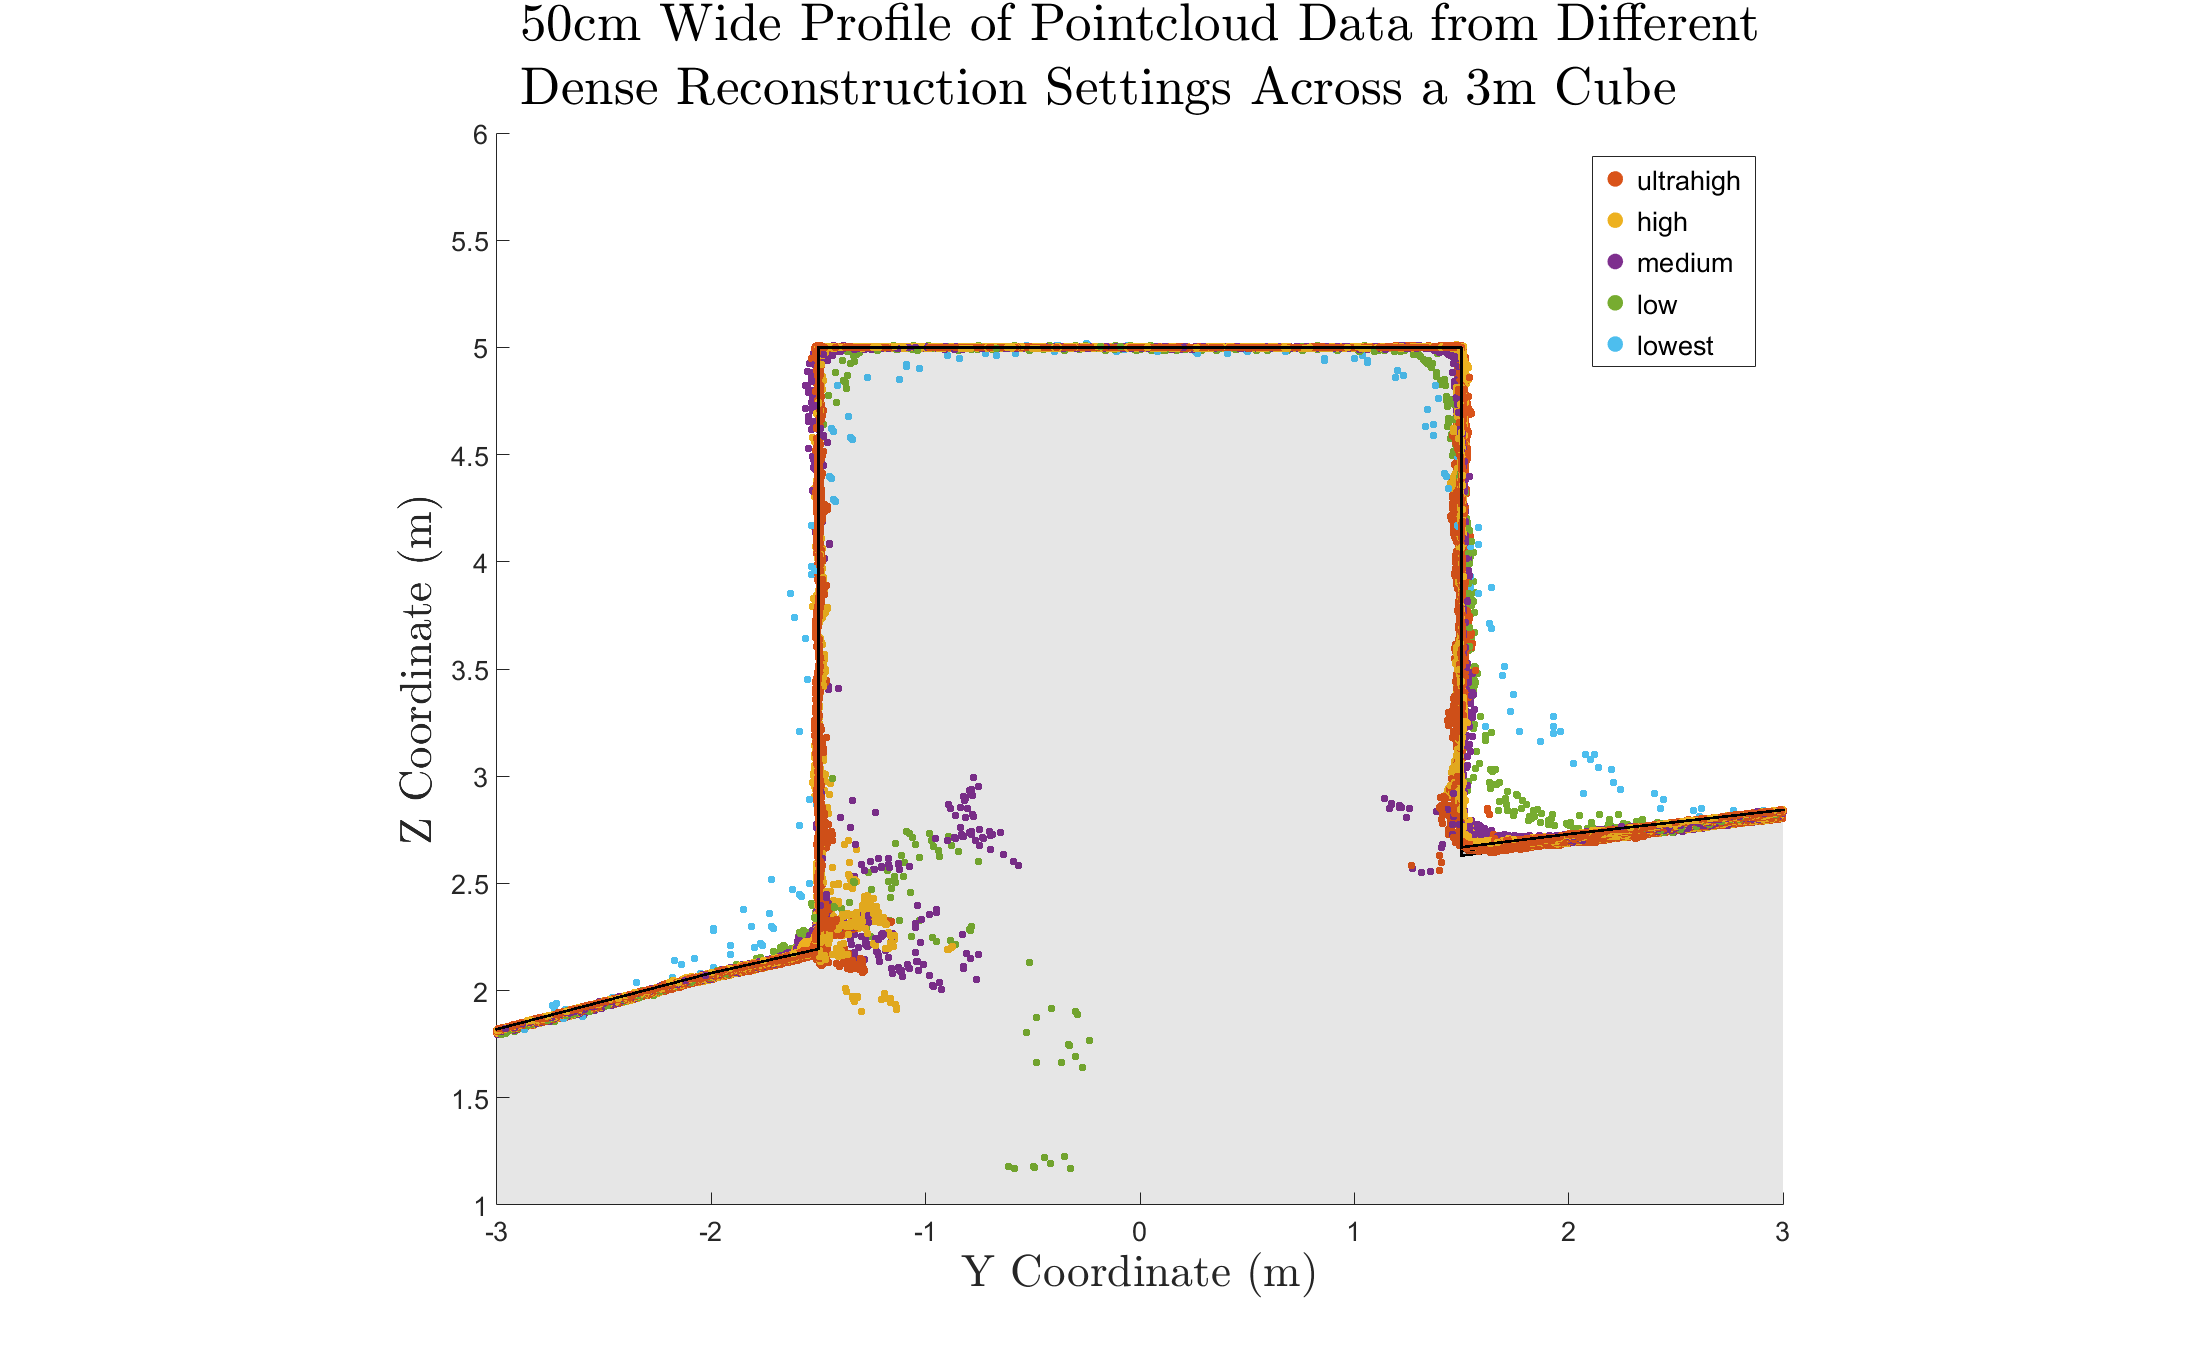
\includegraphics[height = 3in]{../fig/boxprofile}

	\caption{A half meter wide section of the scene containing a box is shown with the dense reconstruction pointclouds overlaid to demonstrate the effect of pointcloud dense reconstruction quality on accuracy near sharp edges.}
	\label{fig:boxplot}
\end{figure}

A more quantitative, statistical assessment is performed to assess the error throughout the entire scene by calculating a histogram for the distribution of error in each pointcloud, as shown in \figref{fig:hist}. These distributions bolster the conclusion derived from the box profile plot, which is that a higher quality dense reconstruction settings yield more accurate results than a lower quality reconstructione.  While the accuracy of the GCPs as provided in Photoscan were an average of 0.38mm RMSE, the accuracy of the dense reconstruction ranges in standard deviation from 2.6mm to 32.3mm.  This observation indicates that the GCP accuracy table is insufficient as a metric to depict the accuracy of the resultant dense pointcloud.  While these conclusions suggest general trends. further experimentation is required in order for the accuracy and magnitudes of the distribution to be generalized.

\begin{figure}[H]
	\centering
	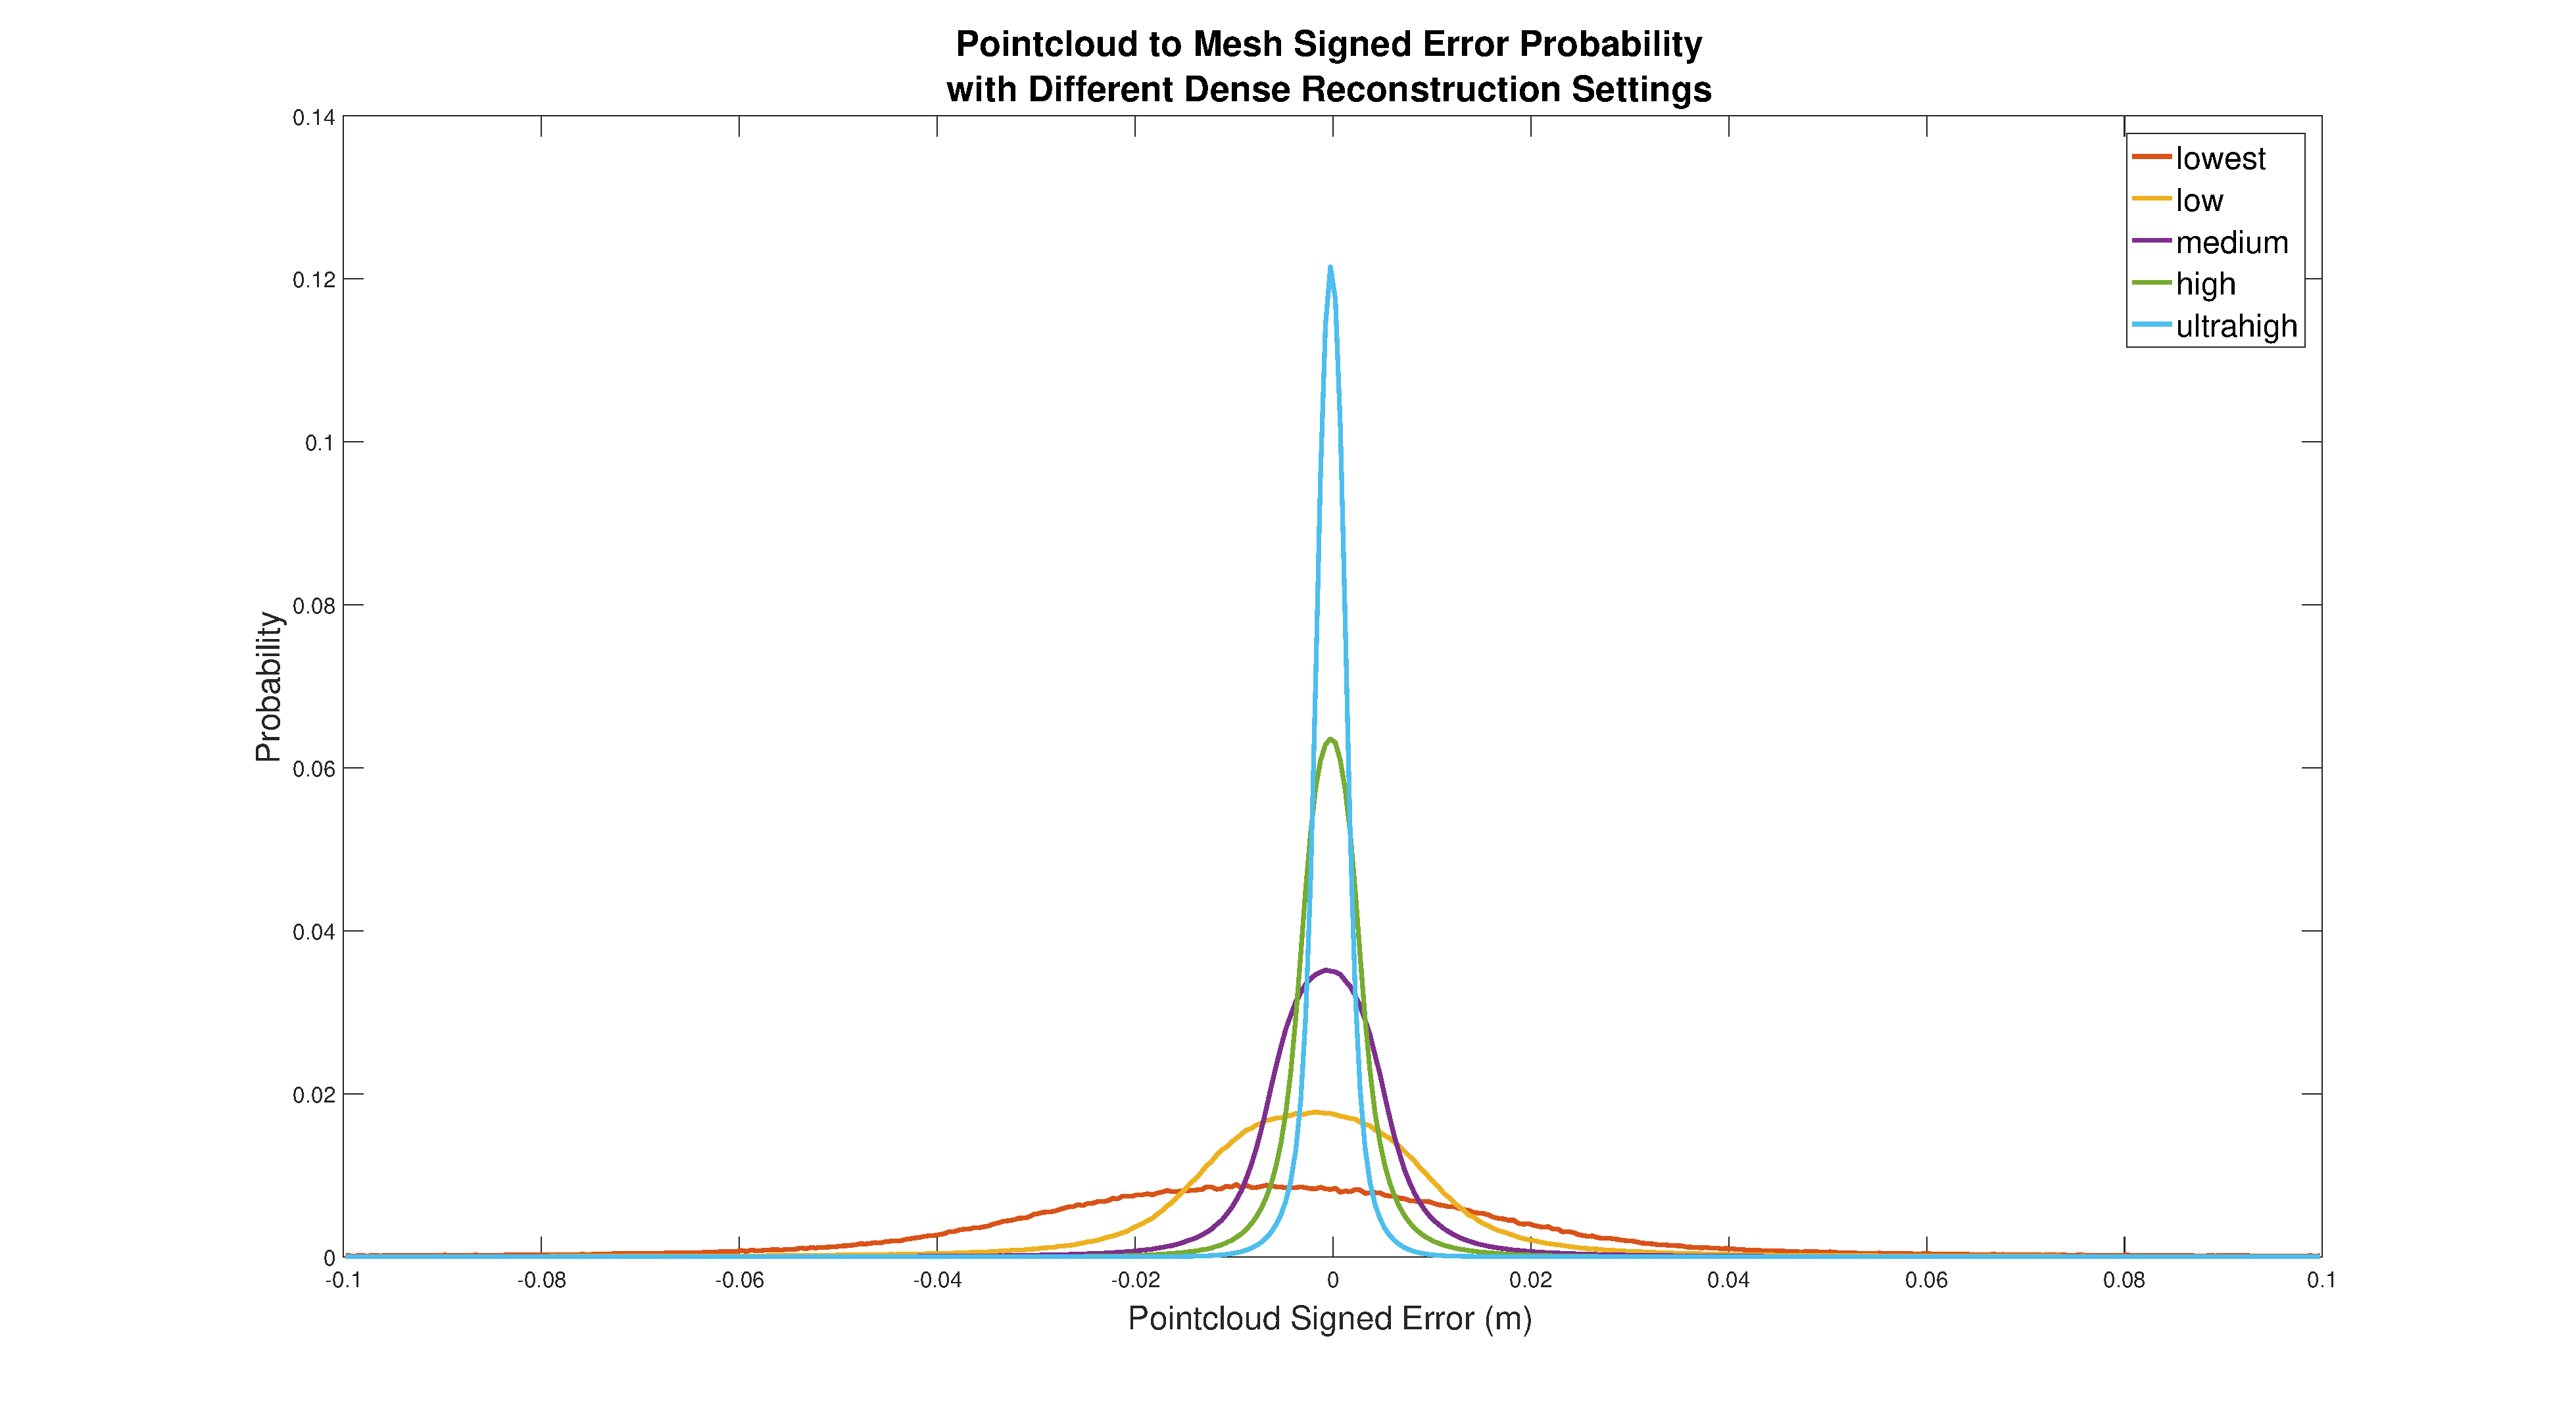
\includegraphics[height = 3in]{../fig/histerror}

	\caption{The signed error probability distribution for each of the calculated dense pointclouds suggests that the higher that dense reconstruction quality, the better the accuracy of the pointcloud.}
	\label{fig:hist}
\end{figure}


%Sourced from Orthophoto AT25. Crown Copyright Reserved. http://www.linz.govt.nz/topography/aerial-images/nztm-geo/bj36
	
